\section{Ejercicio 2}

\subsection{Enunciado}

Ejecutar y graficar la simulación usando el algoritmo \textbf{FCFS} para 1 y 2 y 4 núcleos con un cambio de contexto de 2 ciclos. Calcular la \textit{latencia} de cada tarea en los tres gráficos y el \textit{throughput}.

\begin{center}
	\begin{tabular}{|l|}
		\hline
							\\
		TaskCPU 10			\\
		@5:					\\
		TaskConsola 5 1 4	\\
		@6:					\\
		TaskConsola 5 1 2	\\
		@8:					\\
		TaskCPU 10			\\
							\\
		\hline
	\end{tabular}
\end{center}


\subsection{Resolución}

\begin{figure}[!h]
	\begin{center}
		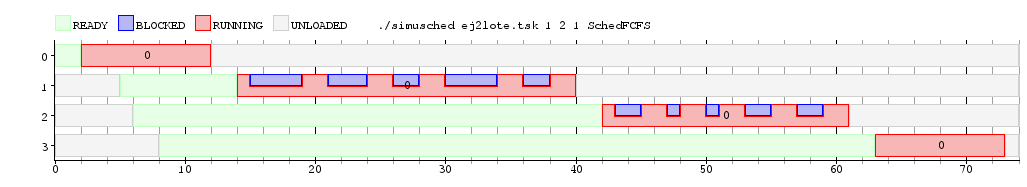
\includegraphics[width=500px]{imagenes/ej2_1.png}
		\caption{\small{\textbf{Grafico generado con el lote usando el algoritmo FCFS para 1 núcleo con un cambio de contexto de 2 ciclos.}}}
		\label{fig:grafico_ej2_1}
	\end{center}
\end{figure}

\begin{figure}[!h]
	\begin{center}
		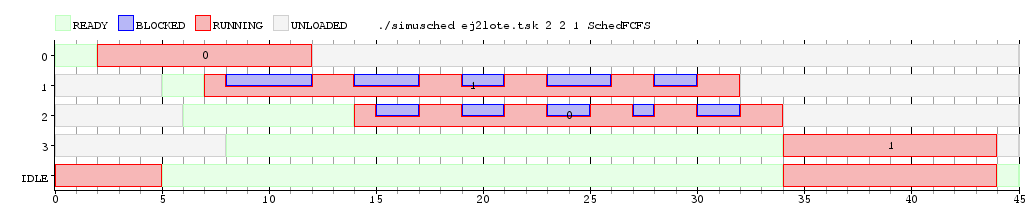
\includegraphics[width=500px]{imagenes/ej2_2.png}
		\caption{\small{\textbf{Grafico generado con el lote usando el algoritmo FCFS para 2 núcleos con un cambio de contexto de 2 ciclos.}}}
		\label{fig:grafico_ej2_2}
	\end{center}
\end{figure}

\begin{figure}[!h]
	\begin{center}
		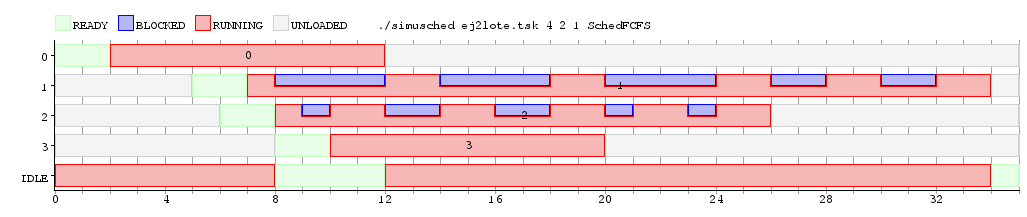
\includegraphics[width=500px]{imagenes/ej2_4.png}
		\caption{\small{\textbf{Grafico generado con el lote usando el algoritmo FCFS para 4 núcleos con un cambio de contexto de 2 ciclos.}}}
		\label{fig:grafico_ej2_4}
	\end{center}
\end{figure}